\documentclass{scrreprt}

\usepackage{aligned-overset}
\usepackage{amsmath}
\usepackage{amssymb}
\usepackage{bm}
\usepackage[shortlabels]{enumitem}
\usepackage{hyperref}
\usepackage[utf8]{inputenc}
\usepackage{mathtools}
\usepackage{physics}
\usepackage{tabularx}
\usepackage{titling}
\usepackage{fancyhdr}
\usepackage{xfrac}
\usepackage{pgfplots}

\definecolor{light-gray}{gray}{.9}

\pgfplotsset{compat = newest}
\usepgfplotslibrary{patchplots}

\usetikzlibrary{intersections}
\usetikzlibrary{patterns}
\usepgfplotslibrary{fillbetween}

\author{Karsten Lehmann}
\date{SoSe 2021}
\title{Übung 08 Analysis - Weiterführende Konzepte}

\pagestyle{fancy}
\fancyhf{}
\lhead{\thetitle}
\rhead{\theauthor}
\lfoot{\thedate}
\rfoot{Seite \thepage}

\newcommand\skalprod[1]{\left\langle #1 \right\rangle}
\newcommand\nnorm[1]{\left\lvert\left\lvert\left\lvert #1 \right\rvert\right\rvert\right\rvert}

\begin{document}
\section*{Partielle Ableitungen}

$f \colon \mathbb{R}^N \to \mathbb{R}^M$ in $x \in \mathbb{R}^N$ differenzierbar
\[
  \iff \exists \: T \in \mathcal{L}\qty(\mathbb{R}^N, \mathbb{R}^M),
  r \colon \mathbb{R}^N \to \mathbb{R}^M \colon f(x + h) =
  f(x) + \underset{f'(x)}{\underbrace{T}}(h) + r(h),
  \frac{r(h)}{\norm{h}} \overset{h \to 0}\longrightarrow 0
\]
\[
  f'(x) \in \mathcal{L}\qty(\mathbb{R}^N, \mathbb{R}^M),
  f' \colon d_f \subseteq \mathbb{R}^N \to \mathcal{L}\qty(\mathbb{R}^N, \mathbb{R}^M)
\]
Auf $\mathbb{R}^N, \mathbb{R}^M$ seien die Standardbasen gegeben.
Dann gibt es genau eine Matrix $A \in \mathbb{R}^{M \times N}$ mit
$y = \underset{\makebox[0pt]{$J_f(x_0)$ Jacobi-Matrix}}{\underbrace{A}} \cdot x$
wobei $x$ Koordinatenvektor von $x$ und $y$ Koordinatenvektor von $f'(x_0)$
bezüglich der Standardbasen ist.

Wir betrachten zunächst $f \colon \mathbb{R}^N \to \mathbb{R}$ und
Richtungsableitungen für $v \in \mathbb{R}^N, v \ne 0$.
Sei $g(t) = f(x_0 + tv), g \colon \mathbb{R} \to \mathbb{R}$.
\begin{flalign*}
  \text{Falls } g'(0) &= \lim_{t \to 0} \frac{1}{t}\qty(g(t) - g(0)) & \\
  &= \lim_{t \to 0} \frac{1}{t} \qty(f(x_0 + tv) - f(x_0)) \text{ existiert,}
\end{flalign*}
wird $d_v f\qty(x_0) \coloneqq \frac{f\qty(x_0)}{dv} = g'(0)$ gesetzt.

Für $v = e_k$ ergeben sich die sogenannten partiellen Ableitungen:
\begin{flalign*}
  \frac{df}{d_{x_x}}\qty(x_0) &= \lim_{t \to 0} \frac{1}{t} \qty(f\qty(x_0 + t_{e_k}) - f\qty(x_0)) & \\
  &= \lim_{t \to 0} \frac{1}{t}
  \qty(\underset{g(t)}{\underbrace{f\qty(x_{0_1}, \ldots, x_{0_{k - 1}}, x_{0_k} + t, x_{0_{k + 1}}, x_{0_N})}}
  - f(x_0))
\end{flalign*}
Falls $f$ in $x_0$ differenzierbar ist, existieren
$\frac{d_f}{d_{x_k}}\qty(x_0), k = 1, \ldots, N$
\[
  D_{f(x)} \coloneqq \qty(\frac{d}{d_{x_1}}, \ldots, \frac{d}{d_{x_N}})f\qty(x_0) \quad\text{(Gradient)}
\]
$\forall h \in \mathbb{R}^N \colon f'\qty(x_0)(h) = \skalprod{D_{f\qty(x_0)}, h}
= \underset{J_f\qty(x_0)}{\underbrace{D_{f\qty(x_0)}^T}} \cdot h$

Zurück zu $f = \qty(_1, \ldots, f_M) \colon \mathbb{R}^N \to \mathbb{R}^M$.
$J_f\qty(x_0) = \begin{pmatrix}
  \frac{d}{d_{x_1}}f_1 & \ldots  & \frac{d}{d_{x_N}}f_1 \\
  \vdots & \vdots & \vdots \\
  \frac{d}{d_{x_1}}f_M & \ldots & \frac{d}{d_{x_N}}f_M
\end{pmatrix}\qty(X_0)$

Die Jacobi-Matrix ist nicht die Ableitung, sondern die Abbildungsmatrix
der Ableitung an der Stelle $x_0$ unter Verwendung der Standardbasen.

\paragraph{Aufgabe 1} Geben Sie von den folgenden Ausdrücken $f(x)$ den größten Bereich
$D(f) \subseteq \mathbb{R}^N$, für den $f$ definiert ist.
Wie lautet der Existenzbereich $D(f') \subseteq D(f)$ der Ableitung $f'$.
Geben Sie die zugehörige Jacobi-Matrix $J_f$ an.
\begin{enumerate}[a)]
\item $f\qty(x_1, x_2) = \sqrt{2x_1 + 3x_1x_2 + 4x_2}$
\item
\item $f\qty(x_1, x_2) = \qty(\tan\qty(x_1) + x_2^4, \ln\qty(x_1 + x_2))$
  \subparagraph{Lsg.} $f \colon D_f \subseteq \mathbb{R}^2 \to \mathbb{R}^2$
  \begin{flalign*}
    f\qty(x_1, x_2) &= \begin{pmatrix}
      \tan\qty(x_1) + x_2^4 \\
      \ln\qty(x_1 + x_2)
    \end{pmatrix} & \\
    \Rightarrow &D_f = \qty{x = \qty(x_1, x_2) \in \mathbb{R}^2 {\Big |}
      \underset{\tan(\ldots)}{\underbrace{x_1 \ne \frac{\pi}{2} + k\pi, k \in \mathbb{Z}}}
      , \underset{\ln(\ldots)}{\underbrace{x_1 + x_2 > 0}}}
    \subseteq \mathbb{R}^2 \: \text{ist eine offene Menge}
  \end{flalign*}
  \[
    x \in D_f \colon J_f (x) = \begin{pmatrix}
      \frac{1}{\cos^2 x_1} & 4 x_2^3 \\
      \frac{1}{x_1 + x_2} & \frac{1}{x_1 + x_2}
    \end{pmatrix}
  \]
  $x \mapsto J_f(x)$ ist stetig auf $D_f = D_{f'} \Rightarrow f$ ist auf
  $D_{f'} = D_f$ stetig differenzierbar.
  \[
    \qty(\text{Die Jacobi-Matrix ist stetig, weil }
     x \mapsto \frac{d_{f_1}(x)}{dx_1}, \frac{d_{f_1}(x)}{dx_2}, \frac{d_{f_2}(x)}{dx_1}, \frac{d_{f_2}(x)}{dx_2},
    \text{ stetig sind})
  \]

\item $f\qty(x_1, x_2) = \qty(x_1, x_2, e^{x_1^2 + 4 x_2})$
  \subparagraph{Lsg.} $f \colon D_f \subseteq \mathbb{R}^2 \to \mathbb{R}^3, D_f = \mathbb{R}^2$
  \[
    f\qty(x_1, x_2) = \begin{pmatrix}
      x_1 \\
      x_2 \\
      e^{x_1^2 + 4x_2}
    \end{pmatrix},
    J_f(x) = \begin{pmatrix}
      1 & 0 \\
      0 & 1 \\
      2 x_1 e^{x_1^2 + 4 x_2} & 4e^{x_1^2 + 4x_2}
    \end{pmatrix}
  \]
  $f$ ist für alle $x \in \mathbb{R}^2$ stetig differenzierbar, da
  $x = \qty(x_1, x_2) \mapsto J_f(x)$ stetig Abbildbar ist.

  \textbf{Achtung:} Generell reicht die Existenz des Gradienten oder der
  Jacobi-Matrix reicht nicht dafür aus, dass die Funktion differenzierbar ist.
  Die Bedingung, dass die Abbildung von $x$ in die Jacobi-Matrix stetig ist, ist
  eine hinreichende Bedingung, dass die Funktion differenzierbar und sogar stetig
  differenzierbar ist.
\end{enumerate}

\newpage
\section*{Tangentialhyperebene und affin-lineare Approximation}
\paragraph{Aufgabe 3} Sei $f \colon D(f) \subseteq \mathbb{R}^N \to \mathbb{R}$
in $x_0 \in D(f)$ differenzierbar.
Dann gibt es eine Funktion $r \colon \mathbb{R}^N$ mit
\[
  f(x_0 + h) = f(x_0) + \skalprod{\nabla f(x_0), h} + r(h) \text{ und }
  \lim_{h \to 0} \frac{r(h)}{\norm{h}} = 0
\]
Damit ist die Funktion
\[
  t_{f,x_0}(x) \coloneqq f(x_0) + \skalprod{\nabla f(x_0), x - x_0}, x \in \mathbb{R}^N
\]
eine affin-lineare Approximation von $f$ in $x_0$.
Dies stellt eine Verallgemeinerung der Tangenten im Fall $N = 1$ dar.
Der Graph der Funktion $t_{f,x_0}$
\[
  \mathbb{T}_{f, x_0} \coloneqq \qty{\qty(x, t_{x_0}(x)) \in \mathbb{R}^{N + 1} {\Big |} x \in \mathbb{R}^N}
  = \qty{(x, y) \in \mathbb{R}^{N + 1} {\Big |} y = f(x_0) + \skalprod{\nabla f(x_0), x - x_0}, x \in \mathbb{R}^N}
\]
wird \textit{Tangentialhyperebene} von $f$ in $x_0$ genannt.
Sie wird von den $N$ Vektoren $\qty(e_k, \partial_k, f(x_0)), k = 1, \ldots, N$
aufgespannt und verläuft durch den Punkt $(x_0, f(x_0))$.
Normalenvektor $n \in \mathbb{R}^{N + 1}$ dieser Ebene ist
\[
  n = (-\nabla f(x_0), 1) \text{ bzw. } n = (\nabla f(x_0), -1)
\]
Damit erlaubt $\mathbb{T}_{f, x_0}$ die Darstellung
\begin{flalign*}
  \mathbb{T}_{f, x_0} &= \qty{(x, y) \in \mathbb{R}^{N + 1} {\Big |} \skalprod{\qty(\nabla f\qty(x_0), -1), (x, y)}
    = \skalprod{(\nabla f \qty(x_0), -1), \qty(x_0, f\qty(x_0))}} & \\
  &= \qty{(x, y) \in \mathbb{R}^{N + 1} {\Big |} \skalprod{n, (x, y)} = \skalprod{n, \qty(x_0, f\qty(x_0))}}
\end{flalign*}
Wobei $\skalprod{., .}$ das Euklidische Skalarprodukt im $\mathbb{R}^{N + 1}$
bezeichnet.
Wir betrachten die Funktion $f \colon \mathbb{R}^2 \to \mathbb{R}$ mit
$f\qty(x_1, x_2) = \sin\qty(x_1 + x_2) - \ln\qty(1 + x_1^2 + x_2^2)$.

\subparagraph{Vorbertrachtung} $f \colon D_f \subseteq \mathbb{R}^N \to \mathbb{R}$
sei in $x_0 \in D_f$ differenzierbar.
\begin{align*}
  \Rightarrow f(\underset{= x}{\underbrace{x_0 + h}})
  &= f\qty(x_0) + \skalprod{\nabla f\qty(x_0), h}
    + r(h) \quad \text{mit } \frac{r(h)}{\norm{h}} \overset{h \to 0}\longrightarrow 0 & \\
  f(x) &= \underset{\makebox[0pt]{$t_{f, x_0}(x)$ affin-lineare lokale Approximation von $f$ in $x_0$}}{
         \underbrace{f\qty(x_0) + \skalprod{\nabla f\qty(x_0), x - x_0}}
         } + \ldots
\end{align*}
($t_{f,x_0}$ ist die Tangente)
\[
  \mathbb{T}_{f, x_0} = \qty{\qty(x, t_{f, x_0}(x)) \in \mathbb{R}^{N + 1} {\Big |} x \in \mathbb{R}^N}
\]
ist Tangential-(hyper)-ebene von $f$ in $x_0$, die von
$\qty(e_k, \frac{df}{dx_x}(x_0)), k = 1, \ldots, N$ aufgespannt wird.
Normalenvektor ist $n = \pm \qty(\nabla f\qty(x_0))$.

\newpage
\begin{enumerate}[a)]
\item Berechnen Sie den Gradienten von $f$.
  Ist $f$ auf $\mathbb{R}^2$ differenzierbar?

  \subparagraph{Lsg.}
  $f\qty(x_1, x_2) = \sin\qty(x_1 + x_2) - \ln\qty(1 + x_1^2 + x_2^2), x \in D_f = \mathbb{R}^2$.
  \[
    \nabla f\qty(x_1, x_2) = \begin{pmatrix}
      \frac{df}{dx_1}(x) \\
      \frac{df}{dx_2}(x)
    \end{pmatrix}
    \underset{\makebox[0pt]{$f\qty(x_1, x_2) = f\qty(x_2, x_1)$}}{\underset{\Big \uparrow}{=}}
    \begin{pmatrix}
      \cos\qty(x_1 + x_2) - \frac{1 \cdot 2 x_1}{1 + x_1^2 + x_2^2} \\
      \cos\qty(x_1 + x_2) - \frac{1 \cdot 2 x_2}{1 + x_1^2 + x_2^2}
    \end{pmatrix}
  \]

  $x \mapsto \nabla f\qty(x_1, x_2)$ ist auf $D_f = \mathbb{R}^2$ stetig.
  $\Rightarrow f$ ist auf $\mathbb{R}^2$ stetig differenzierbar.
  \[
    J_f\qty(x_1, x_2) = \begin{pmatrix}
      \cos\qty(x_1 + x_2) - \frac{2 x_1}{1 + x_1^2 + x_2^2} &
      \cos\qty(x_1 + x_2) - \frac{2 x_2}{1 + x_1^2 + x_2^2}
    \end{pmatrix}
  \]

\item Bestimmen Sie die Tangentialebene von $f$ im Punkt $(1, -1)$.
  \subparagraph{Lsg.}
  \begin{flalign*}
    x_0 = (1, -1) \colon t_{f, x_0} &= f\qty(x_0) + \skalprod{\nabla f\qty(x_0), x - x_0} & \\
    &= f\qty(x_0) + \nabla f(x_0)^T \cdot (x - x_0)
  \end{flalign*}
  Es gilt $f\qty(x_0) = f(1, -1) = -\ln 3, \nabla f\qty(x_0) =
  \nabla f(1, -1) = \qty(1 - \frac{2}{3}, 1 + \frac{2}{3})
  = \qty(\frac{1}{3}, \frac{5}{3})$

  \begin{flalign*}
    t_{f, x_0} (x) &= -\ln 3 + \skalprod{\frac{1}{3}
      \begin{pmatrix}
        1 \\
        5
      \end{pmatrix},
      \frac{x_1 - 1}{x_2 + 1}
    } & \\
    &= -\ln 3 + \frac{1}{3} \qty(\qty(x_1 - 1) + 5 \qty(x_2 + 1)) \\
    &= -\ln 3 + \frac{1}{3} x_1 + \frac{5}{3} x_2 + \frac{4}{3}, x = \qty(x_1, x_2) \in \mathbb{R}^2
  \end{flalign*}
  Taylor-Polynom von $f$ in $x_0$ 1. Ordnung.
  $E = \qty{(x_1, x_2, x_3) {\Big |} \qty(x_1, x_2) \in \mathbb{R}^2, x_3 = t_{f, x_0} \qty(x_1, x_2)}$

 \newpage
\item Geben Sie die Richtungsableitung von $f$ im Punkt $(1, -1)$ in Richtung
  $v \coloneqq \frac{\nabla f(1, -1)}{\norm{\nabla f(1, -1)}_2}$ an.
  \subparagraph{Lsg.} Allgemein: Falls $f$ in $x_0$ differenzierbar ist, gilt
  $\frac{df}{dv} (x_0) = \skalprod{\nabla f\qty(x_0), v} = \nabla f\qty(x_0)^T v \forall v \in \mathbb{R}^N$.
  \[
    v = \frac{\nabla f(1, -1)}{\norm{\nabla f(1, -1)}_2}
    = \frac{\qty(\frac{1}{3}, \frac{5}{3})}{\norm{\qty(\frac{1}{3}, \frac{5}{3})}_2}
    = \frac{\frac{1}{3}(1,5)}{\frac{1}{3} \norm{(1, 5)}_2} = \frac{(1, 5)}{\sqrt{26}}
  \]
  \[
    \Rightarrow \frac{df}{dv} = \skalprod{\nabla f\qty{x_0}, \frac{\nabla f\qty{x_0}}{\norm{\nabla f\qty{x_0}}_2}}
    = \frac{\norm{\nabla f\qty{x_0}}_2^2}{\sqrt{26}}
    = \norm{\nabla f\qty{x_0}}_2 = \norm{\qty(\frac{1}{3}, \frac{5}{3})}_2
    = \frac{1}{3}\sqrt{26}
  \]
  Für $v \in \mathbb{R}^{2(N)}, \norm{v} = 1$ gilt
  $\skalprod{\nabla f\qty(x_0), v} \leq \abs{\skalprod{\nabla f\qty(x_0), v}} \leq \norm{\nabla f\qty(x_0)}_2 \cdot \norm{v}_2$
  $= \norm{\nabla f\qty(x_0)}_2$.

  Frage: Existiert $v_0 \in \mathbb{R}^{2(N)}, \norm{v}_2 = 1$ mit
  $\skalprod{\nabla f\qty(x_0), v_0} = \norm{\nabla f\qty(x_0)}_2$?
  $v_0 = \frac{\nabla f\qty(x_0)}{\norm{\nabla f\qty(x_0)}_2}$ für $\nabla f\qty(x_0) \ne 0$
  (Richtung des steilsten Anstiegs)
\end{enumerate}

\section*{Ketten- und Produktregel}

\paragraph{Aufgabe 4}
\begin{enumerate}[a)]
\item Gegeben seien die Funktionen
  $f, g \colon \mathbb{R}^2 \to \mathbb{R}^2$ mit
  $f(x, y) = (x - y, xy)$ und $g(u, v) = (u^2, v^2 - u^2)$.
  Berechnen Sie die Jacobi-Matrix der verketteten Funktion
  $l = g \circ f \colon \mathbb{R}^2 \to \mathbb{R}^2$
  auf direktem Weg und durch Anwendung der Kettenregel.

  \subparagraph{Lsg.}
  $f, g \colon \mathbb{R}^2 \to \mathbb{R}^2$
  und $f(x, y) = \begin{pmatrix}
    x - y \\
    x \cdot y
  \end{pmatrix},
  g(u, v) = \begin{pmatrix}
    u^2 \\
    v^2 - u^2
  \end{pmatrix}$
  $l \colon \mathbb{R}^2 \to \mathbb{R}^2$ und
  $l(x, y) = (g \circ f) (x, y) = g(f(x, y))$,

  \textbf{direkt:} $l(x, y) = g(x - y, x \cdot y) = \begin{pmatrix}
    (x - y)^2 \\
    (xy)^2 - (x - y)^2
  \end{pmatrix}$
  \[
    J_l(x, y) = \begin{pmatrix}
      2(x - y) & -2 (x - y) \\
      2xy^2 - 2(x - y) & 2x^2y + 2(x - y)
    \end{pmatrix}
  \]
  \textbf{Kettenregel:}
  $J_f (x, y) = \begin{pmatrix}
    1 & -1 \\
    x & y
  \end{pmatrix},
  J_g (u, v) = \begin{pmatrix}
    2u & 0 \\
    -2u & 2v
  \end{pmatrix}$
  \begin{flalign*}
    \Rightarrow J_l (x, y) &= J_g(f(x, y)) \cdot J_f(x, y)
    = J_g(x - y, x \cdot y) \cdot J_f(x, y) & \\
    &= \begin{pmatrix}
      2 (x - y) & 0 \\
      2 (y - x) & 2xy
    \end{pmatrix} \cdot
    \begin{pmatrix}
      1 & -1 \\
      y & x \\
    \end{pmatrix}
    = \begin{pmatrix}
      2 (x - y) & -2 (x - y) \\
      -2 (x - y) + 2xy^2 & 2(x - y) + 2x^2 y
    \end{pmatrix}
  \end{flalign*}

  Alternative Verkettung:
  $k(u, v) = (f \circ g) (u, v) = f(u^2, v^2 - u^2) = \begin{pmatrix}
    u^2 - (v^2 - u^2) \\
    u^2(v^2 - u^2)
  \end{pmatrix} = \begin{pmatrix}
    2u^2 -  v^2 \\
    u^2v^2 - u^4
  \end{pmatrix}, (u,v) \in \mathbb{R}^2$
  \[
    J_k (u, v) = \begin{pmatrix}
      4u & -2v \\
      2uv^2-4u^3 & 2u^2v
    \end{pmatrix}
  \]

\end{enumerate}

\paragraph{Aufgabe 5} Gegeben sei die Funktion
$f \colon \mathbb{R}^2 \to \mathbb{R}$ mit
\[
  f(x) \coloneqq \begin{cases}
    \frac{x_1x_2}{x_1^2 + x_2^2}, & \text{für } x = \qty(x_1, x_2) \ne (0, 0) \\
    0, & \text{für } x = (0, 0)
  \end{cases}
\]

\begin{enumerate}[a)]
\item Untersuchen Sie, ob $f$ im Nullpunkt stetig ist.

  \begin{center}
    \resizebox{.8\textwidth}{!}{
      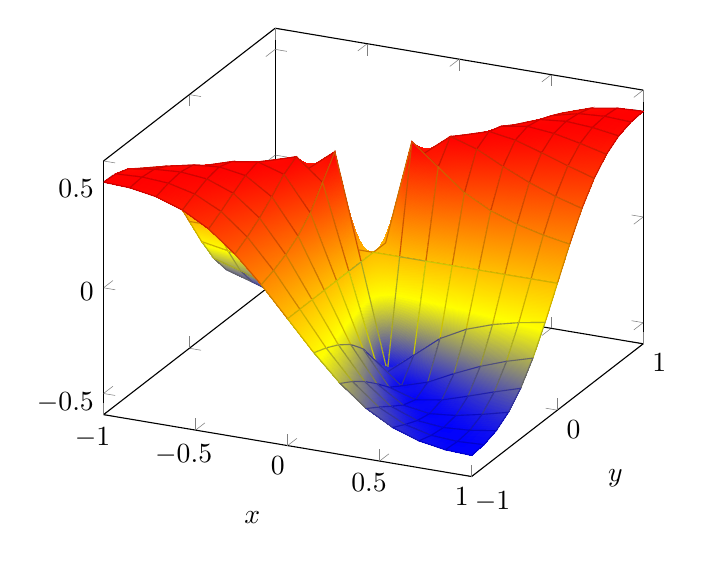
\begin{tikzpicture}[
        declare function={
          f(\x, \y) = \x^2 + \y^2 != 0 ? (\x*\y)/(\x^2 + \y^2) : 0;
        }
        ]
        \begin{axis}[
          xlabel = $x$,
          ylabel = $y$
        ]
          \addplot3[
            surf,
            domain=-1:1,
            samples=15,
            patch type=bilinear,
            shader=faceted interp
          ] {f(x, y)};
        \end{axis}
      \end{tikzpicture}
    }
  \end{center}
  \subparagraph{Lsg.} $M = \mathbb{R}^2 \setminus \qty{0}$ ist offen.
  $f$ ist auf $M$ der Quotient stetig differenzierbarer Funktionen,
  wobei der Nenner ungleich $0$ ist.
  $\Rightarrow f$ ist auf $M$ differenzierbar mit
  \begin{flalign*}
    \frac{df}{dx_1}(x_1, x_2) &= \frac{x_2}{x_1^2 + x_2^2} - \frac{x_1x_2 \cdot 2x_1}{\qty(x_1^2x_2^2)^2}
    = \frac{x_2}{\qty(x_1^2 + x_2^2)^2} \qty\Big(\qty(x_1^2 + x_2^2) - 2x_1^2) & \\
    &= \frac{x_2\qty(x_2^2 - x_1^2)}{\qty(x_1^2 + x_2^2)^2} \\
    \overset{f(x_1, x_2) = f(x_2, x_1)}\Rightarrow \frac{df}{dx_2}(x_1, x_2) &= \frac{x_1\qty(x_1^2 - x_2^2)}{\qty(x_1^2 + x_2^2)^2} \\
    \Rightarrow x = (x_1, x_2) \mapsto \nabla f(x) &= \frac{1}{\qty(x_1^2 + x_2^2)^2} \qty\Big(x_2\qty(x_2^2 - x_1^2), x_1\qty(x_1^2 + x_2^2))
    \text{ ist stetig} \\
    \Rightarrow f \text{ ist auf $M$ stetig differenzierbar}
  \end{flalign*}
  \begin{flalign*}
    \text{Wir betrachten } g(t)
    &= f\qty(t\qty(e_1 + e_2)) = f(t, t) = \frac{t^2}{2t^2} = \frac{1}{2} &\\
    k(t) &= f\qty(t\qty(e_1 - e_2)) = f\qty(t, -t) = -\frac{t^2}{2t^2} = -\frac{1}{2} \\
    \Rightarrow \lim_{t \to 0} g(t) = \frac{1}{2} &\ne \lim_{t \to 0} k(t) = -\frac{1}{2} \\
    \Rightarrow \lim_{(x_1, x_2) \to (0,0)} f(x_1, x_2) &\text{ existiert nicht } \Rightarrow f
    \text{ ist in $(0,0) nicht stetig$}
  \end{flalign*}

\setcounter{enumi}{2}
\item Zeigen Sie, dass die partiellen Ableitungen beliebiger Ordnung von
  $f$ in $(0, 0)$ existieren.
  Warum ist $f$ in $(0, 0)$ trotzdem nicht differenzierbar?

  \subparagraph{Lsg.}
  $g(t) = \overset{f((0,0) + te_1)}{\overset{\downarrow}{f(t, 0)}} = 0 =
  \overset{f((0,0) + te_2)}{\overset{\downarrow}{f(0, t)}}$.

  $\Rightarrow \frac{df}{dx_1}(0, 0) = \frac{df}{dx_2} (0,0) = g'(0) = 0$
  {
    \color{red!60!black}
    \[
      \frac{d^n}{dx_1^n}f(0, 0) = \frac{d^nf}{dx_2^n} (0, 0) = 0
    \]
  }
  Die Funktion ist natürlich trotzdem nicht differenzierbar, den Bedingung für
  die Differenzierbarkeit ist die Stetigkeit.
\end{enumerate}

\end{document}